\documentclass[11pt]{beamer}
\usepackage[utf8]{inputenc}
\usepackage{amsmath}
\usepackage{amsfonts}
\usepackage{amssymb}
\usepackage{amsthm}             
\usepackage{fancyhdr}
\usepackage[english]{babel}
\usepackage{graphicx}
\usepackage{geometry}
\usepackage{tcolorbox}
\usepackage{enumerate}
\usepackage{tikz}
\usepackage{tabularx,colortbl}
\usepackage{empheq}
\usepackage{float}
\usepackage{makecell}
\usepackage[caption = false]{subfig}
\usepackage{cases}
%\usepackage{mdframed}
%\usepackage[driverfallback=hypertex]{hyperref}
%\usepackage{animate}

\graphicspath{{Figure/}} % include path of figure

\newtheorem{definitionkk}[]{Definition}[section]

\setbeamertemplate{caption}[numbered]
%\numberwithin{figure}{section}

\newcommand{\theoremautorefname}{Theorem}
\newcommand{\definitionautorefname}{Definition}
\newcommand{\lemmaautorefname}{Lemma}
\newcommand{\remarkautorefname}{Remark}
\newcommand{\propositionautorefname}{Proposition}
\newcommand{\exampleautorefname}{Example}


\usepackage{mathtools}
\DeclarePairedDelimiter{\abs}{\lvert}{\rvert}  % abs
\DeclarePairedDelimiter{\norm}{\lVert}{\rVert}  % Norm
\DeclarePairedDelimiter{\inner}{\langle}{\rangle} % Inner product

\usetheme{Madrid}
%\usepackage[nodayofweek]{datetime}


\title{Hawkes processes} 
\author{Nguyen Le Thao Trang and Le Thi Minh Phuong}  
\date{\today}

\makeatletter
\setbeamertemplate{footline}
{
	\leavevmode%
	\hbox{%
		\begin{beamercolorbox}[wd=.4\paperwidth,ht=2.25ex,dp=1ex,center]{author in head/foot}%
			\usebeamerfont{author in head/foot}\insertshortauthor
		\end{beamercolorbox}%
		\begin{beamercolorbox}[wd=.3\paperwidth,ht=2.25ex,dp=1ex,center]{title in head/foot}%
			\usebeamerfont{title in head/foot}\insertshorttitle
		\end{beamercolorbox}%
		\begin{beamercolorbox}[wd=.3\paperwidth,ht=2.25ex,dp=1ex,right]{date in head/foot}%
			\usebeamerfont{date in head/foot}\insertshortdate{}\hspace*{2em}
			\insertframenumber{} / \inserttotalframenumber\hspace*{2ex} 
	\end{beamercolorbox}}%
	\vskip0pt%
}
\makeatother

\setbeamertemplate{headline}{}

\setbeamertemplate{lemma}[numbered]
\setbeamertemplate{remark}[numbered]
\setbeamertemplate{example}[numbered]

\usepackage{etoolbox}
\setbeamertemplate{theorems}[numbered]
\undef{\lemma}
\undef{\example}
\newtheorem{lemma}{\translate{Lemma}}
\theoremstyle{example}
\newtheorem{example}{\translate{Example}}

\setbeamercolor{block title example}{fg=white,bg=blue!30!black}
\setbeamercolor{block body example}{fg=black,bg=gray!25!white}
%\AtBeginSubsection[]
%{
%	\begin{frame}<beamer>
%		\frametitle{FDM Schemes For 1D Heat Equation}
%		\tableofcontents[
%		currentsection,
%		sectionstyle=show/show,
%		subsectionstyle=show/shaded/hide
%		]
%	\end{frame}
%}
\usepackage{algorithm,algpseudocode,float}
\floatname{algorithm}{Algorithm}
\renewcommand{\algorithmicrequire}{\textbf{INPUT:}}
\renewcommand{\algorithmicensure}{\textbf{OUTPUT:}}
\makeatletter
\newenvironment{breakablealgorithm}
{% \begin{breakablealgorithm}
	\begin{center}
		\refstepcounter{algorithm}% New algorithm
		\hrule height.8pt depth0pt \kern2pt% \@fs@pre for \@fs@ruled
		\renewcommand{\caption}[2][\relax]{% Make a new \caption
			{\raggedright\textbf{\ALG@name~\thealgorithm} ##2\par}%
			\ifx\relax##1\relax % #1 is \relax
			\addcontentsline{loa}{algorithm}{\protect\numberline{\thealgorithm}##2}%
			\else % #1 is not \relax
			\addcontentsline{loa}{algorithm}{\protect\numberline{\thealgorithm}##1}%
			\fi
			\kern2pt\hrule\kern2pt
		}
	}{% \end{breakablealgorithm}
		\kern2pt\hrule\relax% \@fs@post for \@fs@ruled
	\end{center}
}
\makeatother
\begin{document}
\begin{frame}
	\begin{center}
		\small{\textbf{VIETNAM GENERAL CONFEDERATION OF LABOUR}} \\
		\small{\textbf{TON DUC THANG UNIVERSITY}}\\
		\small{\textbf{FACULTY OF MATHEMATICS AND STATISTICS}} \\
		
		\vspace*{0.2cm}
		
\includegraphics[scale=0.08]{TDT_logo.jpg}
		
		\vspace*{0.2cm}
		\huge{\textbf{HAWKES PROCESSES}}\\
		
		\vspace*{0.5cm}
			\Large{\textit{by}} \\
		\Large{\textbf{Nguyen Le Thao Trang}} \\
		\Large{\textbf{Le Thi Minh Phuong}} \\
		\Large{\textit{advised by}} \\
		\Large{\textbf{Dr. Nguyen Chi Thien}} \\
%		\vspace{2cm}
		
		\vspace*{0.5cm}
		\small
		\text{Ho Chi Minh City, Jun 2019}
	\end{center}	
\end{frame}

\begin{frame}{Outline}
	\tableofcontents
\end{frame}

\section{Introduction}
\begin{frame}{Introduction}
	\begin{figure}[H]
		\centering
		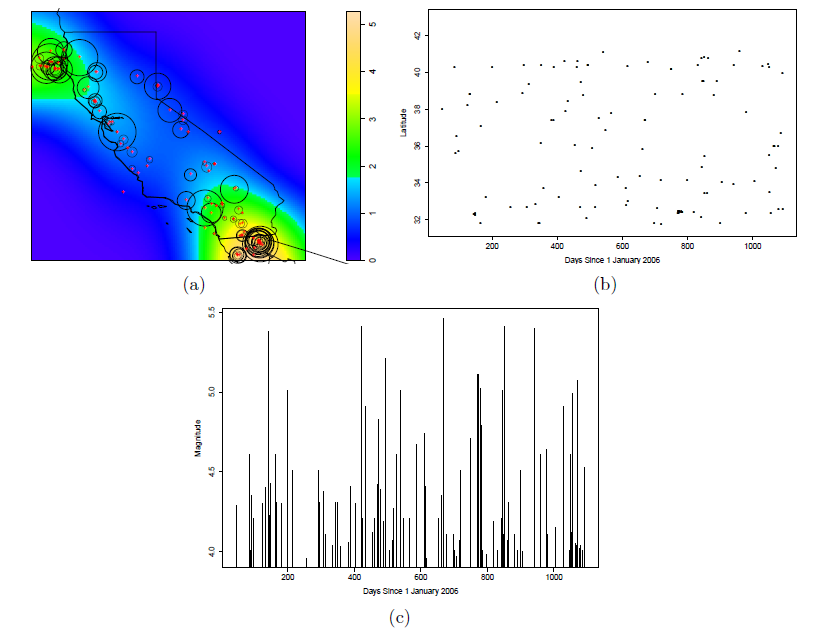
\includegraphics[scale=.5]{introduction}
%		\caption{Seismicity in California during 2006-2008 with magnitude greater than or equal to
%			3.95 on the Richter scale. (a) The red crosses indicate the locations of the events
%			and the circles represent their magnitudes. The color grid shows a kernel intensity
%			estimate on the window. (b) Latitude of event versus occurrence time. (c) Magnitude
%			of event versus occurrence time.}
	\end{figure}
\end{frame}
\section{Background}
\begin{frame}{Background}
\begin{definition}
	\textbf{(Point process)} Let $\{T_i, i \in \mathbb{N} \}$ be a sequence of non-negative random variables such that $\forall i \in \mathbb{N}, T_i<T_{i+1}$. Then $\{T_i, i \in \mathbb{N} \}$ is a (simple) point process.
\end{definition}
\end{frame}
\begin{frame}{Background}
	\begin{definition}
		\textbf{(Counting process)} A counting process is a stochastic process $(N(t):t \geq 0)$ taking values in $\mathbb{N}_0$ that satisfies $N(0)=0$, is almost surely finite, and is a right-continuous step function with increments of size +1. Denote by $(\mathcal{H}(u): u \geq 0)$ the history of the arrivals up to time u.
	\end{definition}
\end{frame}
\begin{frame}{Background}
\begin{figure}[H]
	\centering
	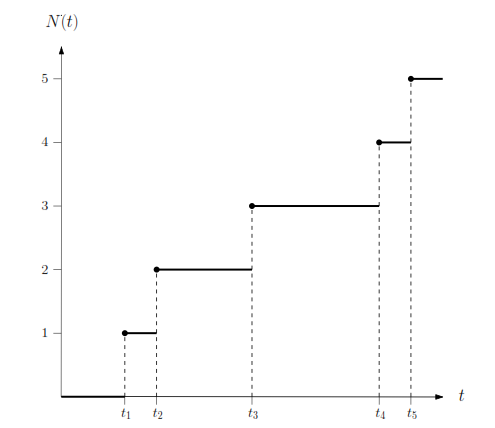
\includegraphics[scale=.6]{coutingprocess}
	\caption[Point process $\{t_1, t_2,...\}$ and corresponding counting process $N(t)$.]{Point process $\{t_1, t_2,...\}$ and corresponding counting process $N(t)$.}
\end{figure}
\end{frame}
%\section{Inhomogeneous Poisson process}
\begin{frame}{Background}
\begin{definition}
	\textbf{(Inhomogeneous Poisson Process)} Consider $(N(t):t \geq 0)$ a counting process and that satisfies
	\begin{align*}
	\mathbb{P}(N(t+h)-N(t)=m|N(t))=
	\begin{cases}
	\lambda(t)h,& \text{if } m=1\\
	o(h) ,& \text{if } m>1\\
	1-\lambda(t)h+o(h),& \text{if } m=0
	\end{cases}
	\end{align*}
	Then $N(t)$ is called a inhomogeneous Poisson process with $\lambda:\mathbb{R}^+ \rightarrow \mathbb{R}^+$.
\end{definition}
\end{frame}
%\section{Hawkes Process}
\begin{frame}{Background}
\begin{definition}
	\textbf{(Hawkes process)} Consider $(N(t):t \geq 0)$ a counting process, with associated history $\mathcal{H}(t):t \geq 0$, that satisfies
	\begin{align*}
	\mathbb{P}(N(t+h)-N(t)=m|\mathcal{H}(t))=
	\begin{cases}
	\lambda^*(t)h+o(h),& \text{if } m=1\\
	o(h) ,& \text{if } m>1\\
	1-\lambda^*(t)h+o(h),& \text{if } m=0
	\end{cases}
	\end{align*}
	Suppose the process' conditional intensity function is of the form
	\begin{align*}
	\lambda^*(t)=\lambda+\int_{0}^{t}\mu(t-u)dN(u)
	\end{align*}
	for some $\lambda>0$ and $\mu:(0,\infty) \rightarrow [0,\infty)$ which are called the background intensity and excitation function respectively. Suppose that $\mu(.) \neq 0$, then a process $N(.)$ is a Hawkes process.
\end{definition}
\end{frame}
\section{Simulation Algorithms}
\begin{frame}{Simulation Algorithms - Inhomogeneous Poisson}
\begin{breakablealgorithm}
		\caption{Generate an inhomogeneous Poisson process by thinning.}
	\label{algorithm:poison}
	\begin{algorithmic}[H]
		\noindent
		\algorithmicrequire{ $T$ is the time to simulate; \\
			\hspace*{1.5 cm}$\lambda(.)$ is the intensity function; \\
			\hspace*{1.5 cm}$M$ is bounded value;}\\
		\algorithmicensure{ The vector $P$ containing the times of occurrences $\{t_1, t_2,...,t_n\}$;}\\
		\textbf{Require:} $\lambda(.) \leq M$ on $[0,T]$.\\
		\textbf{Step 1: } Set $P\leftarrow []$, $t\leftarrow0$\\
		\textbf{Step 2: } while $t<T$ do
		\begin{itemize}
			\item [a.] Generate next candidate point $E \leftarrow$ Exp $(M)$,  $t \leftarrow t+E$
			\item[b.] Keep it with some probability  $U \leftarrow$ Unif$(0,M)$
			\item[c.] if $t <T$ and $U \leq \lambda(t)$ then $P \leftarrow [P,t]$
		\end{itemize}
	\end{algorithmic} 
\end{breakablealgorithm}
\end{frame}
\begin{frame}{Simulation Algorithms - Inhomogeneous Poisson}
	\begin{figure}[H]
		\centering
		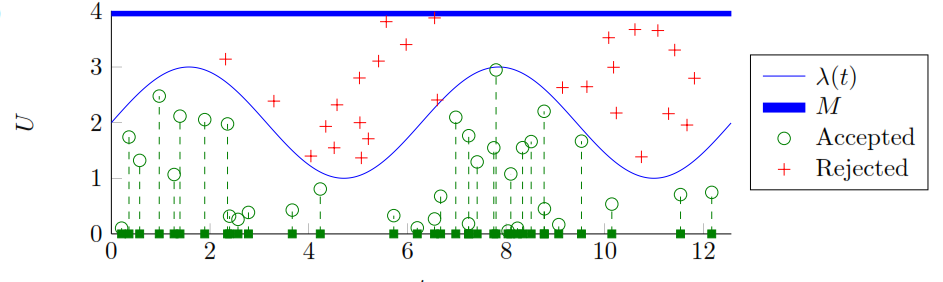
\includegraphics[scale=.45]{poisson}
		\caption{Inhomogeneous Poisson.}
	\end{figure}
\end{frame}
\begin{frame}{Simulation Algorithms - Intensity-based Hawkes Process}
	\begin{breakablealgorithm}
		\caption{Generate a Hawkes process by thinning.}
		\begin{algorithmic}[H]
			\noindent
			\algorithmicrequire{ $T$ is the time to simulate; \\
				\hspace*{1.5 cm}$\lambda^*(.)$ is the conditional intensity function; }\\
			\algorithmicensure{ The vector $P$ containing the times of occurrences $\{t_1, t_2,...,t_n\}$;}\\
			\textbf{Require:} $\lambda^*(.)$ non-increasing in periods without any arrivals.\\
			\textbf{Step 1: } Set $\varepsilon \leftarrow 10^{-10}$, $P\leftarrow[]$, $t\leftarrow0$\\
			\textbf{Step 2: } while $t<T$ do
			\begin{itemize}
				\item [a.] Find new upper bound: $M \leftarrow \lambda^*(t+\varepsilon)$
				\item[b.] Generate next candidate point $E \leftarrow$ Exp$(M)$, $t \leftarrow t+E$
				\item[c.] Keep it with some probability $U \leftarrow$ Unif$(0,M)$
				\item[d.] if $t <T$ and $U \leq \lambda^*(t)$ then $P \leftarrow [P,t]$
			\end{itemize}
		\end{algorithmic} 
	\end{breakablealgorithm}
\end{frame}
\begin{frame}{Simulation Algorithms - Intensity-based Hawkes Process}
	\begin{figure}[H]
		\centering
		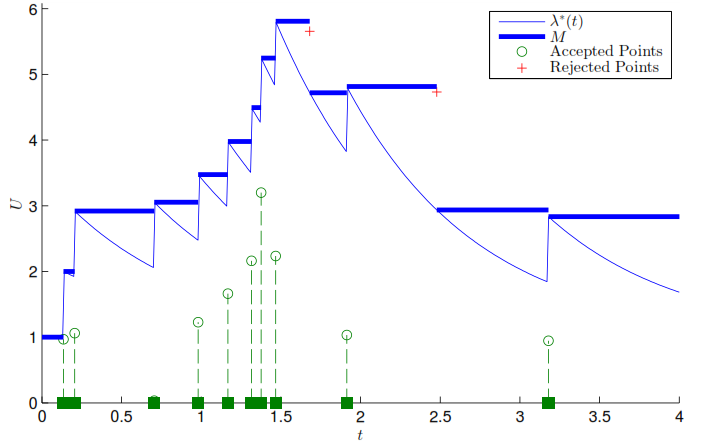
\includegraphics[scale=.45]{hawkesthinning}
		\caption{Intensity-based Hawkes Process.}
	\end{figure}
\end{frame}
\begin{frame}{Simulation Algorithms - Cluster-based Hawkes Process}
\begin{breakablealgorithm}
	\caption{Generate a Hawkes process by clusters.}
	\label{algorithm:hawkescluser}
	\begin{algorithmic}[H]
		\noindent
		\algorithmicrequire{ $T$ is the time to simulate; \\
			\hspace*{1.5 cm} $(\lambda,\alpha,\beta)$ are parameters of the conditional intensity function; }\\
		\algorithmicensure{ $P$ is the union of all the clusters $\{C_1, C_2,...,C_k\}$;}\\
		\textbf{Step 1: } Set $P \leftarrow \{ \}$\\
		\textbf{Step 2: } Generate the immigrants:
		\begin{itemize}
			\item [a.] $k \leftarrow$ Poi$(\lambda T)$
			\item[b.]$C_1, C_2,...,C_k \underleftarrow{\text{ independent and identically distributed}}$ Unif$(0,T)$
		\end{itemize}
		\textbf{Step 3: } Generate the descendants:
		\begin{itemize}
			\item[a.]$D_1, D_2,...,D_k \underleftarrow{\text{ independent and identically distributed}}$ Poi$(\alpha/\beta)$
		\end{itemize}
		\textbf{Step 4: } for $i \leftarrow 1$ to $k$ do\\
		\begin{itemize}
			\item[a.] if $D_i>0$ then
			\begin{itemize}
				\item[a.1] $E_1, E_2,...,E_{D_i} \underleftarrow{\text{ independent and identically distributed}} $ Exp$(\beta)$
				\item[a.2] $P \leftarrow P \cup \{C_i+E_1,C_i+E_2,...,C_i+E_{D_i}\}$
			\end{itemize}
		\end{itemize}
\end{algorithmic} 
	\end{breakablealgorithm}
\end{frame}
\begin{frame}{Simulation Algorithms - Cluster-based Hawkes Process}
				\noindent
	\hspace*{.5cm}	\textbf{Step 5: } Remove descendant outside $[0,T]$
		\begin{align*}
		P \leftarrow \{P_i:P_i \in P,P_i \leq T \}
		\end{align*}
		\hspace*{.5cm} \textbf{Step 6: } Add in immigrants and sort:
		$P \leftarrow$ Sort $(P \cup \{C_1, C_2,...,C_k \})$

\end{frame}
\begin{frame}{Simulation Algorithms - Cluster-based Hawkes Process}
	\begin{figure}[H]
		\centering
		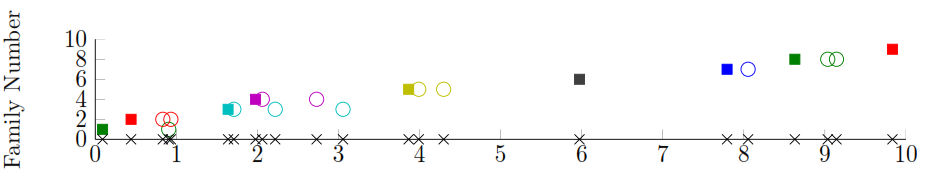
\includegraphics[scale=.45]{hawkescluser}
		\caption{Cluster-based Hawkes Process.}
	\end{figure}
\end{frame}

%\begin{frame}
%	The idea behind using this model is that earthquakes cause aftershocks - this is reflected in the fact that every new earthquake increases the intensity by $\alpha e^{\beta_{\kappa_i}}$.Note that large earthquakes increase the intensity more than small earthquakes. Note that this model does not have independent marks, since the intensity depends on the past marks.
%\end{frame}
\begin{frame}
	\begin{center}
		\Huge{\textbf{THANK YOU!}}
	\end{center}	
\end{frame}
\end{document}